%%%%%%%%%%%%%%%%%%%%%%%%%%%%%%%%%%%%%%%%%
% Beamer Presentation
% LaTeX Template
% Version 1.0 (10/11/12)
%
% This template has been downloaded from:
% http://www.LaTeXTemplates.com
%
% License:
% CC BY-NC-SA 3.0 (http://creativecommons.org/licenses/by-nc-sa/3.0/)
%
%%%%%%%%%%%%%%%%%%%%%%%%%%%%%%%%%%%%%%%%%

%----------------------------------------------------------------------------------------
%	PACKAGES AND THEMES
%----------------------------------------------------------------------------------------

\documentclass[12pt]{beamer}
\mode<presentation> {

% The Beamer class comes with a number of default slide themes
% which change the colors and layouts of slides. Below this is a list
% of all the themes, uncomment each in turn to see what they look like.

%\usetheme{default}
%\usetheme{AnnArbor}
%\usetheme{Antibes}
%\usetheme{Bergen}
%\usetheme{Berkeley}
%\usetheme{Berlin}
%\usetheme{Boadilla}
%\usetheme{CambridgeUS}
%\usetheme{Copenhagen}
%\usetheme{Darmstadt}
%\usetheme{Dresden}
%\usetheme{Frankfurt}
%\usetheme{Goettingen}
%\usetheme{Hannover}
%\usetheme{Ilmenau}
%\usetheme{JuanLesPins}
%\usetheme{Luebeck}
%\usetheme{Madrid}
%\usetheme{Malmoe}
%\usetheme{Marburg}
%\usetheme{Montpellier}
%\usetheme{PaloAlto}
%\usetheme{Pittsburgh}
%\usetheme{Rochester}
%\usetheme{Singapore}
%\usetheme{Szeged}
\usetheme{Warsaw}

% As well as themes, the Beamer class has a number of color themes
% for any slide theme. Uncomment each of these in turn to see how it
% changes the colors of your current slide theme.

%\usecolortheme{albatross}
%\usecolortheme{beaver}
%\usecolortheme{beetle}
%\usecolortheme{crane}
%\usecolortheme{dolphin}
%\usecolortheme{dove}
%\usecolortheme{fly}
%\usecolortheme{lily}
%\usecolortheme{orchid}
%\usecolortheme{rose}
%\usecolortheme{seagull}
%\usecolortheme{seahorse}
%\usecolortheme{whale}
%\usecolortheme{wolverine}

%\setbeamertemplate{footline} % To remove the footer line in all slides uncomment this line
%\setbeamertemplate{footline}[page number] % To replace the footer line in all slides with a simple
%slide count uncomment this line

\setbeamertemplate{navigation symbols}{} % To remove the navigation symbols from the bottom of all
%slides uncomment this line
}
\expandafter\def\expandafter\insertshorttitle\expandafter{%
  \insertshorttitle\hfill%
  \insertframenumber\,/\,\inserttotalframenumber}

\usepackage{algorithm,algorithmic}
\usepackage{graphicx} % Allows including images
\usepackage{booktabs} % Allows the use of \toprule, \midrule and \bottomrule in tables
\usepackage{tikz}
\usepackage{color}
\usepackage{tkz-graph}
\usepackage[utf8]{inputenc}
\usepackage[danish]{babel}
\usepackage{mathtools}% Loads amsmath
\usepackage{amsmath}
\usetikzlibrary{decorations.pathreplacing}	

% \usetikzlibrary{arrows,decorations.pathmorphing,backgrounds,positioning,fit,matrix} 
% \tikzstyle{vertex}=[circle,fill=black!25,minimum size=15pt,inner sep=0pt]
% \tikzstyle{selectedvertex} = [vertex, fill=red!24] 
% \tikzstyle{edge} = [draw,thick,-] 
% \tikzstyle{arc}= [draw,thick,->,shorten >=1pt,>=stealth'] 
% \tikzstyle{arcl} = [draw,thick,->,shorten>=1pt,>=stealth',bend left=25] 
% \tikzstyle{arcr} = [draw,thick,->,shorten >=1pt,>=stealth']
% \tikzstyle{rpath}=[draw, thick,->,shorten >=1pt,>=stealth',red, opacity=0.4]
% \tikzstyle{weight} = [font=\small] 
% \tikzstyle{selected edge} = [draw,line width=5pt,-,red!50]
% \tikzstyle{ignored edge} = [draw,line width=5pt,-,black!20] 
% \newcommand*{\vpointer}{\vcenter{\hbox{\scalebox{2}{\Huge\pointer}}}}	
% \def\Arrow{\raisebox{3\height}{\scalebox{3}{$\Rightarrow$}}}
\tikzstyle{arc}= [draw,thick,->,shorten >=1pt,>=stealth'] 
%\tikzstyle{vertex}=[circle,fill=black!25,minimum size=15pt,inner sep=0pt]
\tikzstyle{vertex}=[circle, draw, inner sep=0pt, minimum size=10pt]
\newcommand{\vertex}{\node[vertex]}
\def\Arrow{{\scalebox{2}{$\Rightarrow$}}}

%----------------------------------------------------------------------------------------
%	TITLE PAGE
%----------------------------------------------------------------------------------------

\title[]{Et Lokalsøgningssystem til at Løse Diskrete 
Optimeringsproblemer}% The short title appears at 
%the bottom of every slide, the full title is only on the title page

\author{Bo Stentebjerg-Hansen} % Your name
\institute[IMADA] % Your institution as it will appear on the bottom of every slide, may be
%shorthand %to save space
{
Syddansk Universitet \\ % Your institution for the title page
\medskip
Institut for Matematik og Datalogi
%\textit{IMADA} % Your email address
}
\date{\today} % Date, can be changed to a custom date

\begin{document}

\begin{frame}
\titlepage % Print the title page as the first slide
\end{frame}

\begin{frame}
\frametitle{Overblik} % Table of contents slide, comment this block out to remove it
\tableofcontents % Throughout your presentation, if you choose to use \section{} and \subsection{}
%commands, these will automatically be printed on this slide as an overview of your presentation
\end{frame}

%----------------------------------------------------------------------------------------
%	PRESENTATION SLIDES
%----------------------------------------------------------------------------------------

%------------------------------------------------
\section{Introduktion} % Sections can be created in order to organize your presentation into
%discrete blocks, all sections and subsections are automatically printed in the table of contents as
%an overview of the talk
%------------------------------------------------
%\subsection{Subsection Example} % A subsection can be created just before a set of slides with a
%common theme to further break down your presentation into chunks

\begin{frame}
\frametitle{Introduktion}
\begin{itemize}[<+->]
\item 
\item 
\end{itemize}




\end{frame}

%------------------------------------------------	
%\section{Definition af problemer}
\begin{frame}
\frametitle{Binære optimeringsproblemer}
\begin{align}
 \text{Minimize }\; &z =  \mathbf{c}^T\mathbf{x} \\ 
 \text{subject to } \; & \mathbf{A}\mathbf{x} \leq \mathbf{b} \\ 
 & \mathbf{x} \in \{0,1\}^n
\end{align} \noindent
$\mathbf{A}$ er en $m \times n$ matrice, $\mathbf{c}$ og $\mathbf{b}$ er $n$ dimensionale vectorer, alle tre består af 
heltal. $\mathbf{x}$ er en $n$ dimensional vector bestående af binære variable.   
\end{frame}

%------------------------------------------------

\begin{frame}
\frametitle{Eksempel}
% \begin{align}
%  \text{Minimize }\; z =  2&x_1 + x_2 + x_3\\ 
%  \text{subject to } \;  - &x_1 + 2x_2 \leq 1 \\
%  & x_1 +x_2 + x_3 = 2 \\
%  & \mathbf{x} \in \{0,1\}^3
% \end{align} \noindent
\begin{table}[]
\begin{center}
\label{my-label}
\begin{tabular}{llrcrlrl}
Minimize   & z = & $2x_1$        & +  & $x_2$       & + & $x_3$ &          \\
subject to &     & $-x_1$        & + & $2x_2$      &   &       & $\leq 1$  \\
           &     & $x_1$         & + & $x_2$       & + & $x_3$ & $=2$     
               
\end{tabular}
\end{center}
$\qquad \qquad $  $x_1,x_2,x_3 $  $\in$ $\{0,1\}$ 
\end{table}
En mulig løsning: \\
\vspace{0.2cm}
\begin{minipage}{0.47\linewidth}
 $x_1 = 1$  \\
 $x_2 = 0$ \\ 
 $x_3 = 1$ \\
\end{minipage}
\begin{minipage}{0.47\linewidth}

 $z = 2\cdot 1 + 1\cdot 0 + 1\cdot 1  =3$ \\
\end{minipage}
\end{frame}

%------------------------------------------------

\section{Løsningsmetoder}
\begin{frame}
\frametitle{Helttals programmering}
\begin{itemize}[<+->]  
\item Simplex metode.
\item Ligningsbaseret model.
\item Kan ikke altid finde en (optimal) løsning inden for rimelig tid.
\item Gurobi, GLPK, SCIP.
\end{itemize}
\begin{center}
\end{center}
\end{frame}

%------------------------------------------------

\begin{frame}
\frametitle{Constraint programming}
\begin{itemize}[<+->]
\item Bruger søgetræer til at finde en løsning.
\item Mere naturlig formulering af problemer.
\item bl.a. Gecode, prolog.
\end{itemize}
% \begin{center}
\end{frame}

\begin{frame}
\frametitle{Lokal søgning}
\begin{itemize}[<+->]
\item Ændre få variable ad gangen og ser beregner effekten.
\item Kan undersøge mange mulige løsninger.
\item Kan ikke garantere optimalitet.
\item Ofte implementeret til specifikke problemer.
\end{itemize}
% \begin{center}
\end{frame}


\begin{frame}
\frametitle{Constraint programming med lokalsøgning}
\begin{itemize}[<+->]
\item Formulering af problem som i Constraint programming. 
\item Genanvendelse af algoritmer.
\item Giver mulighed for at fokusere på modellering.
\item Solver fx Comet og OscaR.
\end{itemize}
% \begin{center}
\end{frame}


\begin{frame}
\frametitle{Hvad er gjort i det her projekt}
\begin{itemize}[<+->] 
\item Kombinere Gecode og lokal søgning.
\item Undersøger effekten af Gecode. 
\item Tester brugen af invarianter. 
\item Introducerer en ny evalueringsmetode.
\end{itemize}
\end{frame}


%------------------------------------------------
% \section{Finding a maximal matching}
%------------------------------------------------


%------------------------------------------------
\section{Opbygning af systemet}

\begin{frame}
\frametitle{Overblik}
\begin{itemize}[<+->] 
\item Objekter, en kasse med værktøj og information. 
\item Brugerflade og to delt system. 
\end{itemize}
Her er et flot billed af formulering -> GPSolver -> GecodeEngine -> LocalSearcEngine. 

\end{frame}


\begin{frame}
\frametitle{Start løsning - GecodeEngine}
\begin{itemize}[<+->]
\pause 
\item Opret variable og begrænsninger.
\item Preprocessering af Gecode.
\item Oprettelse af søgningsstrategi. 
\item Finder måske en gyldig løsning.
\end{itemize}
\end{frame}

%------------------------------------------------
\begin{frame}
\frametitle{Forberedelse til lokalsøgning}
\begin{itemize}[<+->]
\item Definer variable ud fra betingelser hvis muligt.
\item Graf over afhængighed.
\item Betingelser lavet som invarianter.
\item Ordning af invarianter.
\end{itemize}
\end{frame}

%------------------------------------------------

\begin{frame}
\frametitle{Uafhængige variable gjort afhængige}
\begin{itemize}[<+->]
\item Færre mulige løsninger der skal undersøges.
\item Bruger lidt mere tid på at evaluere en løsning.
\item $x_1 +x_2 -x_3 = 1$.
\item $x_3 = x_1 +x_2 -1$.
\item $x_3$ er gjort afhængig af $x_1$ og $x_2$. 
\item Fjerner betingelsen da den altid vil være overholdt.
\end{itemize}

\end{frame}

%------------------------------------------------


\begin{frame}
\frametitle{Graf over afhængigheder}
\begin{itemize}[<+->]
 \item $x_3 = x_1 +x_2 -1$.
 \item $x_4 = x_3 + x_5 - 1$.
\end{itemize}
\onslide<3-6>
 \begin{minipage}{0.3\linewidth}
% \begin{figure}
     \centering
     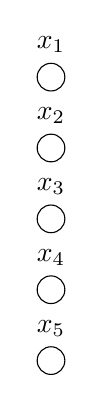
\begin{tikzpicture}[scale=0.9]
        \vertex[label=$x_1$](x1) at (0,4) {};
        \vertex[label=$x_2$](x2) at (0,3) {};
        \vertex[label=$x_3$](x3) at (0,2) {};
        \vertex[label=$x_4$](x4) at (0,1) {};
        \vertex[label=$x_5$](x5) at (0,0) {};
            \end{tikzpicture}
 \end{minipage}
 \onslide<4-6>
\Arrow
%   \onslide<4-5>
% \visible<4-5>
    \begin{minipage}{0.5\linewidth}
    \centering
  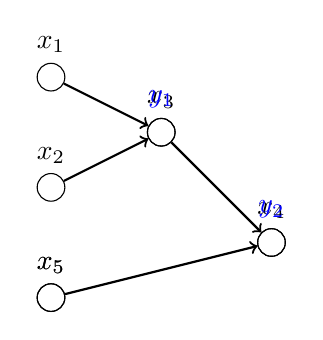
\begin{tikzpicture}[scale=0.7]
          \onslide<4-6>{\vertex[label=$x_1$](x1) at (0,4) {};}
           \onslide<4-6>{\vertex[label=$x_2$](x2) at (0,2) {};}
           \onslide<5-6>{\vertex[label=$x_5$](x5) at (0,0) {};}
           \onslide<4-5>{\vertex[label=$x_3$](i1) at (2,3) {};}
           \onslide<5>{\vertex[label=$x_4$](i2) at (4,1) {};}
      \tikzset{EdgeStyle/.style={->}}
           \onslide<4-6>{\Edge(x1)(i1)}
           \onslide<4-6>{\Edge(x2)(i1)}
           \onslide<5-6>{\Edge(i1)(i2)}
           \onslide<5-6>{\Edge(x5)(i2)}
          %        \begin{tikzpicture}[scale=0.7]
%             \onslide<5>{\vertex[label=$x_1$](x1) at (0,4) {};}
%              \onslide<5>{\vertex[label=$x_2$](x2) at (0,2) {};}
             \onslide<5-6>{\vertex[label=$x_5$](x5) at (0,0) {};}
             \onslide<6>{\vertex[label= \color{blue}$y_1$](i1) at (2,3) {};}
             \onslide<6>{\vertex[label= \color{blue}$y_2$](i2) at (4,1) {};}
        \tikzset{EdgeStyle/.style={->}}
%              \onslide<5-6>{\Edge(x1)(i1)}
%              \onslide<5-6>{\Edge(x2)(i1)}
%              \onslide<6>{\Edge(i1)(i2)}
%              \onslide<6>{\Edge(x5)(i2)}
      \end{tikzpicture}
   \end{minipage}
\end{frame}

%------------------------------------------------
\begin{frame}
\frametitle{Problemer med kredse}
\pause
 \begin{minipage}{0.47\linewidth}
  $y_1 = x_1 - y_3$ \\
  $y_2 = y_1 $ \\
  $y_3 = x_3 +y_2-1$  \\
  $x_1,x_2,y_1,y_2,y_3 \in \{0,1\}$
 \end{minipage}
 \begingroup
    \fontsize{9pt}{12pt}\selectfont
 \begin{minipage}{0.47\linewidth}
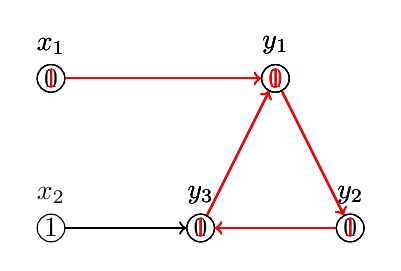
\begin{tikzpicture}[scale=1.9]
        \onslide<3>{\vertex[label=$x_1$](x1) at (0,1) {0};}
        \onslide<5-8>{\vertex[label=$x_1$](x1) at (0,1) {1};}
        \onslide<3-8>{\vertex[label=$x_2$](x2) at (0,0) {1};}
        \onslide<3-4>{\vertex[label=$y_1$](y1) at (1.5,1) {0};}
        \onslide<6-7>{\vertex[label=$y_1$](y1) at (1.5,1) {1};}
        \onslide<3-5>{\vertex[label=$y_2$](y2) at (2,0) {0};}
        \onslide<7-8>{\vertex[label=$y_2$](y2) at (2,0) {1};}
        \onslide<3-6>{\vertex[label=$y_3$](y3) at (1,0) {0};}
        \onslide<8>{\vertex[label=$y_3$](y3) at (1,0) {1};}
        \onslide<4>{\vertex[label=$x_1$](x1) at (0,1) {\color{red}1};}
        \onslide<5>{\vertex[label=$y_1$](y1) at (1.5,1) {\color{red}1};}
        \onslide<8>{\vertex[label=$y_1$](y1) at (1.5,1) {\color{red}0};}
        \onslide<6>{\vertex[label=$y_2$](y2) at (2,0) {\color{red}1};}
        \onslide<7>{\vertex[label=$y_3$](y3) at (1,0) {\color{red}1};}
        \tikzset{EdgeStyle/.style={->}}
             \onslide<3,5-8>{\Edge(x1)(y1)}
             \onslide<3-4,6-8>{\Edge(y1)(y2)}
             \onslide<3-5,7-8>{\Edge(y2)(y3)}
             \onslide<3-6,8>{\Edge(y3)(y1)}
             \onslide<3-8>{\Edge(x2)(y3)}
             %
             \onslide<4>{\Edge[style={color=red}](x1)(y1)}
             \onslide<5,8>{\Edge[style={color=red}](y1)(y2)}
             \onslide<6>{\Edge[style={color=red}](y2)(y3)}
             \onslide<7>{\Edge[style={color=red}](y3)(y1)}
             %\onslide<3-7>{\Edge[style={color=red}](x2)(y3)}
      \end{tikzpicture}
   \end{minipage}
\endgroup
\end{frame}
%-------------------------------------------------------
 \begin{frame}
 \frametitle{Identificering af kredse}
 \begin{itemize}[<+->]
  \item Dybde først lignende algoritme, af Tarjan. 
  \item Finder stærke sammenhængskomponenter (SCC). 
  \item Genopretter en betingelse og variable fra hver SCC.
  \item Gentager indtil ingen stærke sammenhængskomponenter er fundet. 
\end{itemize}
\end{frame}


%-------------------------------------------------------
 \begin{frame}
 \frametitle{Identificering af kredse}
 \begin{minipage}{0.4\linewidth}
  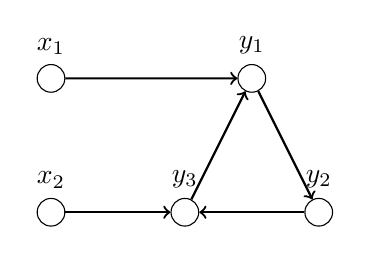
\begin{tikzpicture}[scale=1.7]
%  \onslide<3>{\vertex[label=$x_1$](x1) at (0,1) {0};}
        \onslide<1-3>{\vertex[label=$x_1$](x1) at (0,1) {};}
         \onslide<1-3>{\vertex[label=$x_2$](x2) at (0,0) {};}
        \onslide<1-3>{\vertex[label=$y_1$](y1) at (1.5,1) {};}
%         \onslide<>{\vertex[label=$y_1$](y1) at (1,1) {1};}
        \onslide<1-3>{\vertex[label=$y_2$](y2) at (2,0) {};}
%         \onslide<7-8>{\vertex[label=$y_2$](y2) at (2,1) {1};}
        \onslide<1-3>{\vertex[label=$y_3$](y3) at (1,0) {};}
        \tikzset{EdgeStyle/.style={->}}
             \onslide<1-3>{\Edge(x1)(y1)}
             \onslide<1-3>{\Edge(y1)(y2)}
             \onslide<1-3>{\Edge(y2)(y3)}
             \onslide<1-3>{\Edge(y3)(y1)}
             \onslide<1-3>{\Edge(x2)(y3)}
  \end{tikzpicture}
  \end{minipage}
  \onslide<2-3>
  \Arrow \hfill
     \begin{minipage}{0.45\linewidth}
    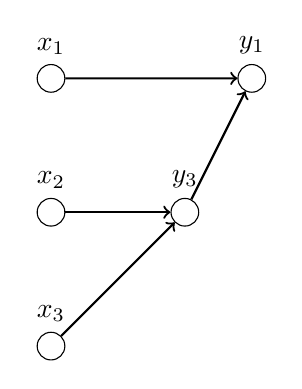
\begin{tikzpicture}[scale=1.7]
 \onslide<2-3>{\vertex[label=$x_1$](x1) at (0,1) {};}
         \onslide<2-3>{\vertex[label=$x_2$](x2) at (0,0) {};}
         \onslide<2-3>{\vertex[label=$x_3$](x3) at (0,-1) {};}
         \onslide<2-3>{\vertex[label=$y_1$](y1) at (1.5,1) {};}
%         \onslide<>{\vertex[label=$y_1$](y1) at (1,1) {1};}
%         \onslide<2-3>{\vertex[label=$y_2$](y2) at (2,1) {};}
%         \onslide<7-8>{\vertex[label=$y_2$](y2) at (2,1) {1};}
        \onslide<2-3>{\vertex[label=$y_3$](y3) at (1,0) {};}
        \tikzset{EdgeStyle/.style={->}}
              \onslide<2-3>{\Edge(x1)(y1)}
              \onslide<2-3>{\Edge(x3)(y3)}
%              \onslide<2-3>{\Edge(y2)(y3)}
              \onslide<2-3>{\Edge(y3)(y1)}
             \onslide<2-3>{\Edge(x2)(y3)}
  \end{tikzpicture}  
  \end{minipage}
  
  \onslide<3>
  \begin{itemize}[<+->]
   \item Genindfører variablen $x_3$ og betingelsen.
   \item $ y_2 = y_1 \Leftrightarrow y_1 -x_3  =0$.
  \end{itemize}

\end{frame}

%------------------------------------------------
\begin{frame}
\frametitle{Forberedelse til lokalsøgning}
\begin{itemize}
\item Definer variable ud fra betingelser hvis muligt.
\item Graf over afhængighed.
\item \textbf{Betingelser lavet som invarianter.}
\item Ordning af invarianter.
\end{itemize}
\end{frame}

%------------------------------------------------
 \begin{frame}
 \frametitle{Betingelser erstattet af invarianter}
 \begin{itemize}[<+->]
  \item Betingelser som ikke er brugt til at definere variable. 
  \item Betingelses specifik oprettelse af invarianter.
  \item Tilføj invarianter til grafen. 
  \item Linear betingelsen opretter to invarianter.
  \item Invarianter til summering af overtrædelse betingelser.
\end{itemize}
 
 \end{frame}


%------------------------------------------------

\begin{frame}
 \frametitle{Invarianter for linear}
 \begin{itemize}[<+->]
  \item Summering af venstresiden: $\;\underbrace{x_1 + 2x_2 -x_3}_{y_1} \leq 2$
  \item Overtrædelse af betingelsen: $\; \underbrace{y_1 \leq 2}_{y_2} \;, $
\end{itemize}
     $\qquad \qquad y_2 = \begin{cases}
        y_1-2, & \text{if $y_1> 2$}.\\
        0, & \text{otherwise}.
       \end{cases}$
\end{frame}
%-----------------------------------------------------
\begin{frame}
 \frametitle{Endelige graf}
   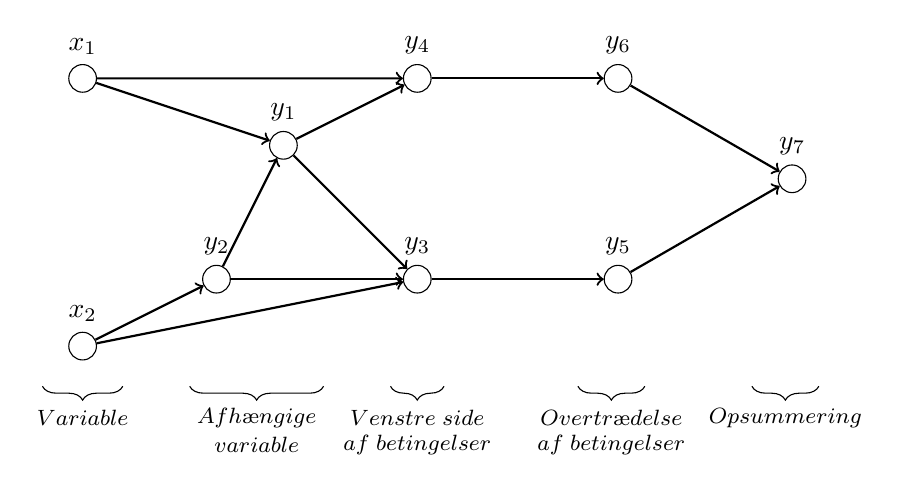
\begin{tikzpicture}[scale=1.7]
   \draw [decorate,decoration={brace,amplitude=5pt},xshift=-0pt,yshift=-0pt,rotate=270]
   (0.8,0.3) -- (0.8,-0.3) node [black,midway,yshift=-0.4cm] 
{\footnotesize $Variable$};
\onslide<2-5>{
   \draw [decorate,decoration={brace,amplitude=5pt},xshift=-0pt,yshift=-0pt,rotate=270]
   (0.8,1.8) -- (0.8,0.8) node [black,midway,yshift=-0.4cm] 
{\footnotesize $Afhængige$};
   \draw [decorate,decoration={brace,amplitude=5pt},xshift=-0pt,yshift=-0pt,rotate=270]
   (1,1.3) -- (1,1.3) node [black,midway,yshift=-0.4cm] 
{\footnotesize $variable$};
}
\onslide<3-5>{
   \draw [decorate,decoration={brace,amplitude=5pt},xshift=-0pt,yshift=-0pt,rotate=270]
   (0.8,2.7) -- (0.8,2.3) node [black,midway,yshift=-0.4cm] 
{\footnotesize $Venstre\; side$};
   \draw [decorate,decoration={brace,amplitude=5pt},xshift=-0pt,yshift=-0pt,rotate=270]
   (1,2.5) -- (1,2.5) node [black,midway,yshift=-0.4cm] 
   {\footnotesize $af\; betingelser$};
   }
   \onslide<4-5>{
    
   
\draw [decorate,decoration={brace,amplitude=5pt},xshift=-0pt,yshift=-0pt,rotate=270]
   (0.8,4.2) -- (0.8,3.7) node [black,midway,yshift=-0.4cm] 
   {\footnotesize $Overtrædelse$};
      \draw [decorate,decoration={brace,amplitude=5pt},xshift=-0pt,yshift=-0pt,rotate=270]
   (1,3.95) -- (1,3.95) node [black,midway,yshift=-0.4cm] 
   {\footnotesize $af\; betingelser$};
   }
   \onslide<5>{
   \draw [decorate,decoration={brace,amplitude=5pt},xshift=-0pt,yshift=-0pt,rotate=270]
   (0.8,5.5) -- (0.8,5) node [black,midway,yshift=-0.4cm] 
   {\footnotesize $Opsumm	ering$};
   }
         \onslide<1-5>{\vertex[label=$x_1$](x1) at (0,1.5) {};}
          \onslide<1-5>{\vertex[label=$x_2$](x2) at (0,-.5) {};}
         \onslide<2-5>{\vertex[label=$y_1$](y1) at (1.5,1) {};}
         \onslide<3-5>{\vertex[label=$y_3$](y2) at (2.5,0) {};}
         \onslide<2-5>{\vertex[label=$y_2$](y3) at (1,0) {};}
         \onslide<3-5>{\vertex[label=$y_4$](y4) at (2.5,1.5) {};}
         \onslide<4-5>{\vertex[label=$y_5$](y5) at (4,0) {};}
         \onslide<4-5>{\vertex[label=$y_6$](y6) at (4,1.5) {};}
         \onslide<5>{\vertex[label=$y_7$](y7) at (5.3,0.75) {};}
         \tikzset{EdgeStyle/.style={->}}
              \onslide<2-5>{\Edge(x1)(y1)}
              \onslide<3-5>{\Edge(y1)(y2)}
              \onslide<3-5>{\Edge(x1)(y4)}
              \onslide<3-5>{\Edge(y1)(y4)}
              \onslide<3-5>{\Edge(y3)(y2)}
              \onslide<2-5>{\Edge(y3)(y1)}
              \onslide<2-5>{\Edge(x2)(y3)}
              \onslide<3-5>{\Edge(x2)(y2)}
	      \onslide<4-5>{\Edge(y4)(y6)}
              \onslide<4-5>{\Edge(y2)(y5)}
              \onslide<5>{\Edge(y5)(y7)}
              \onslide<5>{\Edge(y6)(y7)}
   \end{tikzpicture}
 \end{frame}


%------------------------------------------------
\begin{frame}
\frametitle{Forberedelse til lokalsøgning}
\begin{itemize}
\item Definer variable ud fra betingelser hvis muligt.
\item Graf over afhængighed.
\item Betingelser omdannet til invarianter.
\item \textbf{Ordning af invarianter.}
\end{itemize}
\end{frame}

%----------------------------------------------------------------------------------------

\begin{frame}
\frametitle{Ordning af invarianter}
\begin{itemize}
\item Lav ordning af invarianter til når de skal opdateres. 
\item Forhindre flere opdateringer af samme invariant.
\item Ordningen kan laves med dybde først søgning i grafen.
\item Opret en liste for hver uafhængig variable. 
\end{itemize}
\end{frame}

%----------------------------------------------------------------------------------------

\begin{frame}
\frametitle{Eksempel for en variable}
\centering
% \begin{figure}[!t]
% \centering
% 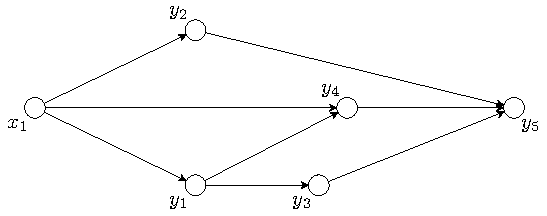
\includegraphics[width=0.6\linewidth]{1.pdf} 
% % \end{center} 
% \end{figure}%
\begingroup
\begin{center}
    \fontsize{9pt}{12pt}\selectfont
  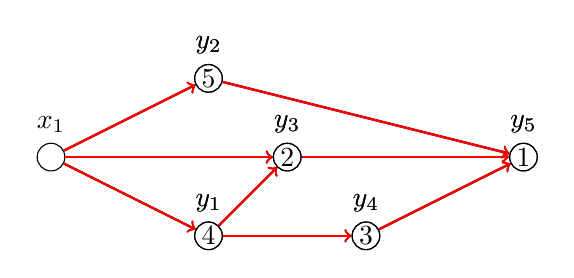
\begin{tikzpicture}[scale=1]
        \onslide<1-16>{\vertex[label=$x_1$](x1) at (0,1) { };}
         \onslide<1-9>{\vertex[label=$y_1$](y1) at (2,0) { };}
        \onslide<1-13>{\vertex[label=$y_2$](y2) at (2,2) { };}
        \onslide<1-5>{\vertex[label=$y_3$](y3) at (3,1) { };}
        \onslide<1-8>{\vertex[label=$y_4$](y4) at (4,0) {};}
        \onslide<1-4>{\vertex[label=$y_5$](y5) at (6,1) {};}
        \tikzset{EdgeStyle/.style={->}}
             \onslide<1,3-16>{\Edge(x1)(y1)}
             \onslide<1-11,13,15,16>{\Edge(x1)(y2)}
             \onslide<1-10,12-16>{\Edge(x1)(y3)}
             \onslide<1-6,8,10-16>{\Edge(y1)(y4)}
             \onslide<1-2,4,5,7-16>{\Edge(y1)(y3)}
             \onslide<1-12,14-16>{\Edge(y2)(y5)}
             \onslide<1-3,6-16>{\Edge(y3)(y5)}
             \onslide<1-7,9-16>{\Edge(y4)(y5)}
%         \onslide<13>{\vertex[label=$x_1$](x1') at (0,1) {};}

        \onslide<10-16>{\vertex[label=$y_1$](y1') at (2,0) {4};}
        \onslide<14-16>{\vertex[label=$y_2$](y2') at (2,2) {5};}
        \onslide<6-16>{\vertex[label=$y_3$](y3') at (3,1) {2};}
        \onslide<9-16>{\vertex[label=$y_4$](y4') at (4,0) {3};}
        \onslide<5-16>{\vertex[label=$y_5$](y5') at (6,1) {1};}
        \tikzset{EdgeStyle/.style={->}}
             \onslide<2,10>{\Edge[style={color=red}](x1)(y1)}
             \onslide<12,14>{\Edge[style={color=red}](x1)(y2)}
             \onslide<11>{\Edge[style={color=red}](x1)(y3)}
             \onslide<7,9>{\Edge[style={color=red}](y1)(y4)}
             \onslide<3,6>{\Edge[style={color=red}](y1)(y3)}
             \onslide<13>{\Edge[style={color=red}](y2)(y5)}
             \onslide<4,5>{\Edge[style={color=red}](y3)(y5)}
             \onslide<8>{\Edge[style={color=red}](y4)(y5)}
  \end{tikzpicture}
  \onslide<16>
    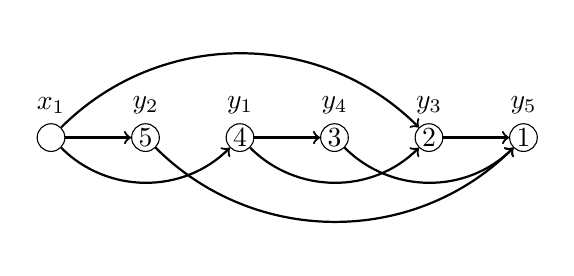
\begin{tikzpicture}[scale=1.2]
        \vertex[label=$x_1$](x1) at (0,0) {};
        \vertex[label=$y_1$](y1) at (2,0) {4};
        \vertex[label=$y_2$](y2) at (1,0) {5};
        \vertex[label=$y_3$](y3) at (4,0) {2};
        \vertex[label=$y_4$](y4) at (3,0) {3};
        \vertex[label=$y_5$](y5) at (5,0) {1};
        \tikzset{EdgeStyle/.style={->}}
           \Edge[style={bend right = 45}](x1)(y1)
           \Edge[style={bend right = 0}](x1)(y2)
           \Edge[style={bend left = 45}](x1)(y3)
           \Edge[style={bend right = 0}](y1)(y4)
           \Edge[style={bend right = 45}](y1)(y3)
           \Edge[style={bend right = 45}](y2)(y5)
           \Edge[style={bend right = 0}](y3)(y5)
           \Edge[style={bend right = 45}](y4)(y5)
  \end{tikzpicture}
  \end{center}

\endgroup
\end{frame}




%----------------------------------------------------------------------------------------
\section{Lokalsøgning}
\begin{frame}
\frametitle{}
\begin{itemize}
\item
\end{itemize}
\end{frame}









\end{document}